%% ID: prism
%% TITLE: Prism
%% TYPE: question
%% QUESTIONTYPE:  scq
%% CONCEPTS: forces, vectors1, newtoni, newtonii, newtoniii
%% VIDEOS: 
%% LEVEL: 5
%% TOPIC: mechanics/statics
%% ORDER: 3

%Nice problem, all it requires is resolving forces but confuses a lot of people. 
\begin{problem}[Tripos_prism_friction_adapted] 
 {\question{The prism (whose cross section is an isosceles triangle) shown in Figure \ref{fig:Statics_prismq} has a mass of \valuedef{m}{0.1}{kg}, and you wish to lift it, touching the upper two faces only.  If the coefficient of friction between the prism's surface and your skin is \valuedef{\mu}{0.4}{}, how hard must you push directly against each face in order to support the prism?
\begin{figure}[h]
\centering
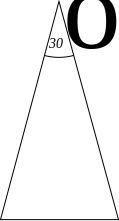
\includegraphics[width=2.3cm]{../../../figures/Statics_prismq.svg}
\caption{}
\label{fig:Statics_prismq}
\end{figure}}

\begin{enumerate}
\item \choice[a]{\quantity{3.85}{N}}\correct
\item \choice[b]{\quantity{0.51}{N}}
\item \choice[c]{\quantity{4.74}{N}}
\item \choice[d]{\quantity{0.85}{N}}
\item \choice[e]{\quantity{1.27}{N}}
\end{enumerate}
}
{\textit{Used with permission from Cambridge University Tripos, Physics Paper 1A, Question A4.}}
{\answer{The correct answer is (a)}
Figure \ref{fig:Statics_prisma} shows the forces acting on the body:
\begin{figure}[h]
\centering
\includegraphics[width=5.5cm]{Statics_prisma}
\caption{}
\label{fig:Statics_prisma}
\end{figure}
\\
Resolving vertically we have
\begin{align*}
2F_2\cos{15}=2F_1\sin{15}+mg
\end{align*}
We also know that $F_1$ and $F_2$ are related. By Newton's third law, $F_1$ will be equal to the reaction force, so on the point of slipping
\begin{align*}
F_2&=\mu F_1 \\
\Rightarrow 2\mu F_1\cos{15}&=2F_1\sin{15}+mg \\
\Rightarrow 2F_1\left(\mu\cos{15}-\sin{15}\right)&=mg \\
\Rightarrow F_1&=\frac{mg}{2\left(\mu\cos{15}-\sin{15}\right)}
\end{align*}
The minimum force required is therefore 3.85 N. 
}
\end{problem}